\chapter{Конструкторская часть}
В этом разделе будет представлено описание используемых типов данных, а также схемы алгоритма полного перебора и муравьиного алгоритма.

\section{Требования к программному обеспечению}

К программе предъявлен ряд требований:
\begin{enumerate}[label=\arabic*)]
	\item программа должна получать на вход матрицу смежности, для которой можно будет выбрать один из алгоритмов поиска оптимальных путей (полным перебором или муравьиным алгоритмом);
	\item программа должна давать возможность получить минимальную сумму пути, а также сам путь, используя один из алгоритмов;
	\item программа должна иметь возможность провести параметризацию муравьиного алгоритма, а также замерить процессорное время работы реализаций алгоритмов.
\end{enumerate}

\section{Разработка алгоритмов}
На рисунке \ref{fig:full} представлена схема алгоритма полного перебора путей, а на рисунках \ref{fig:ant} и \ref{fig:ant2} схема муравьиного алгоритма поиска путей. Также на рисунках \ref{fig:ant_choose} и \ref{fig:ant_phero} представлены схемы вспомогательных функций для муравьиного алгоритма.

\begin{figure}[h!]
	\centering
	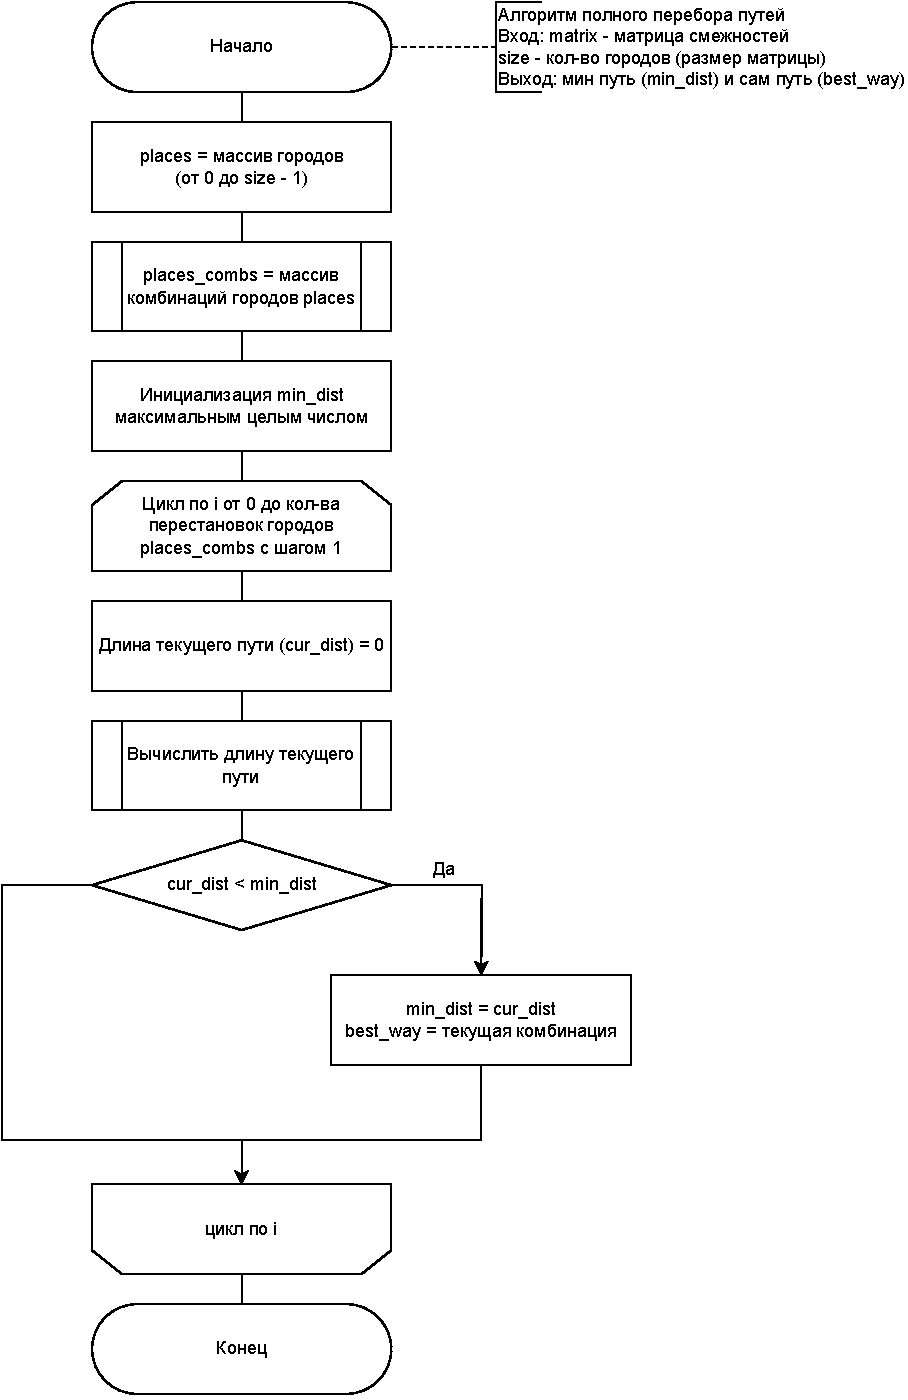
\includegraphics[width=0.95\linewidth]{img/full}
	\caption{Схема алгоритма полного перебора путей}
	\label{fig:full}
\end{figure}
\begin{figure}[h!]
	\centering
	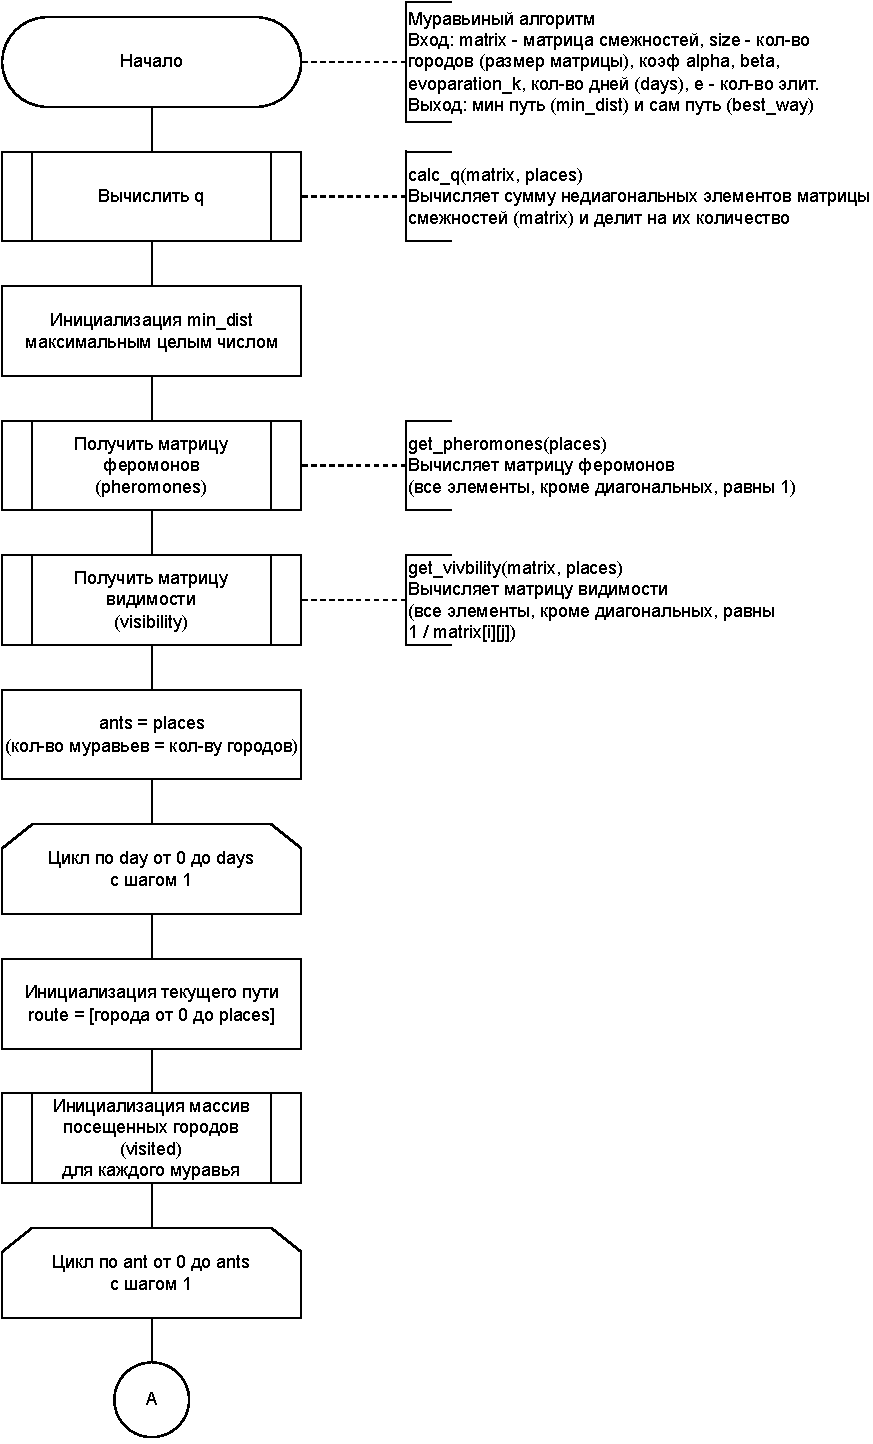
\includegraphics[width=0.9\linewidth]{img/ant}
	\caption{Схема муравьиного алгоритма (часть 1)}
	\label{fig:ant}
\end{figure}
\begin{figure}[h!]
	\centering
	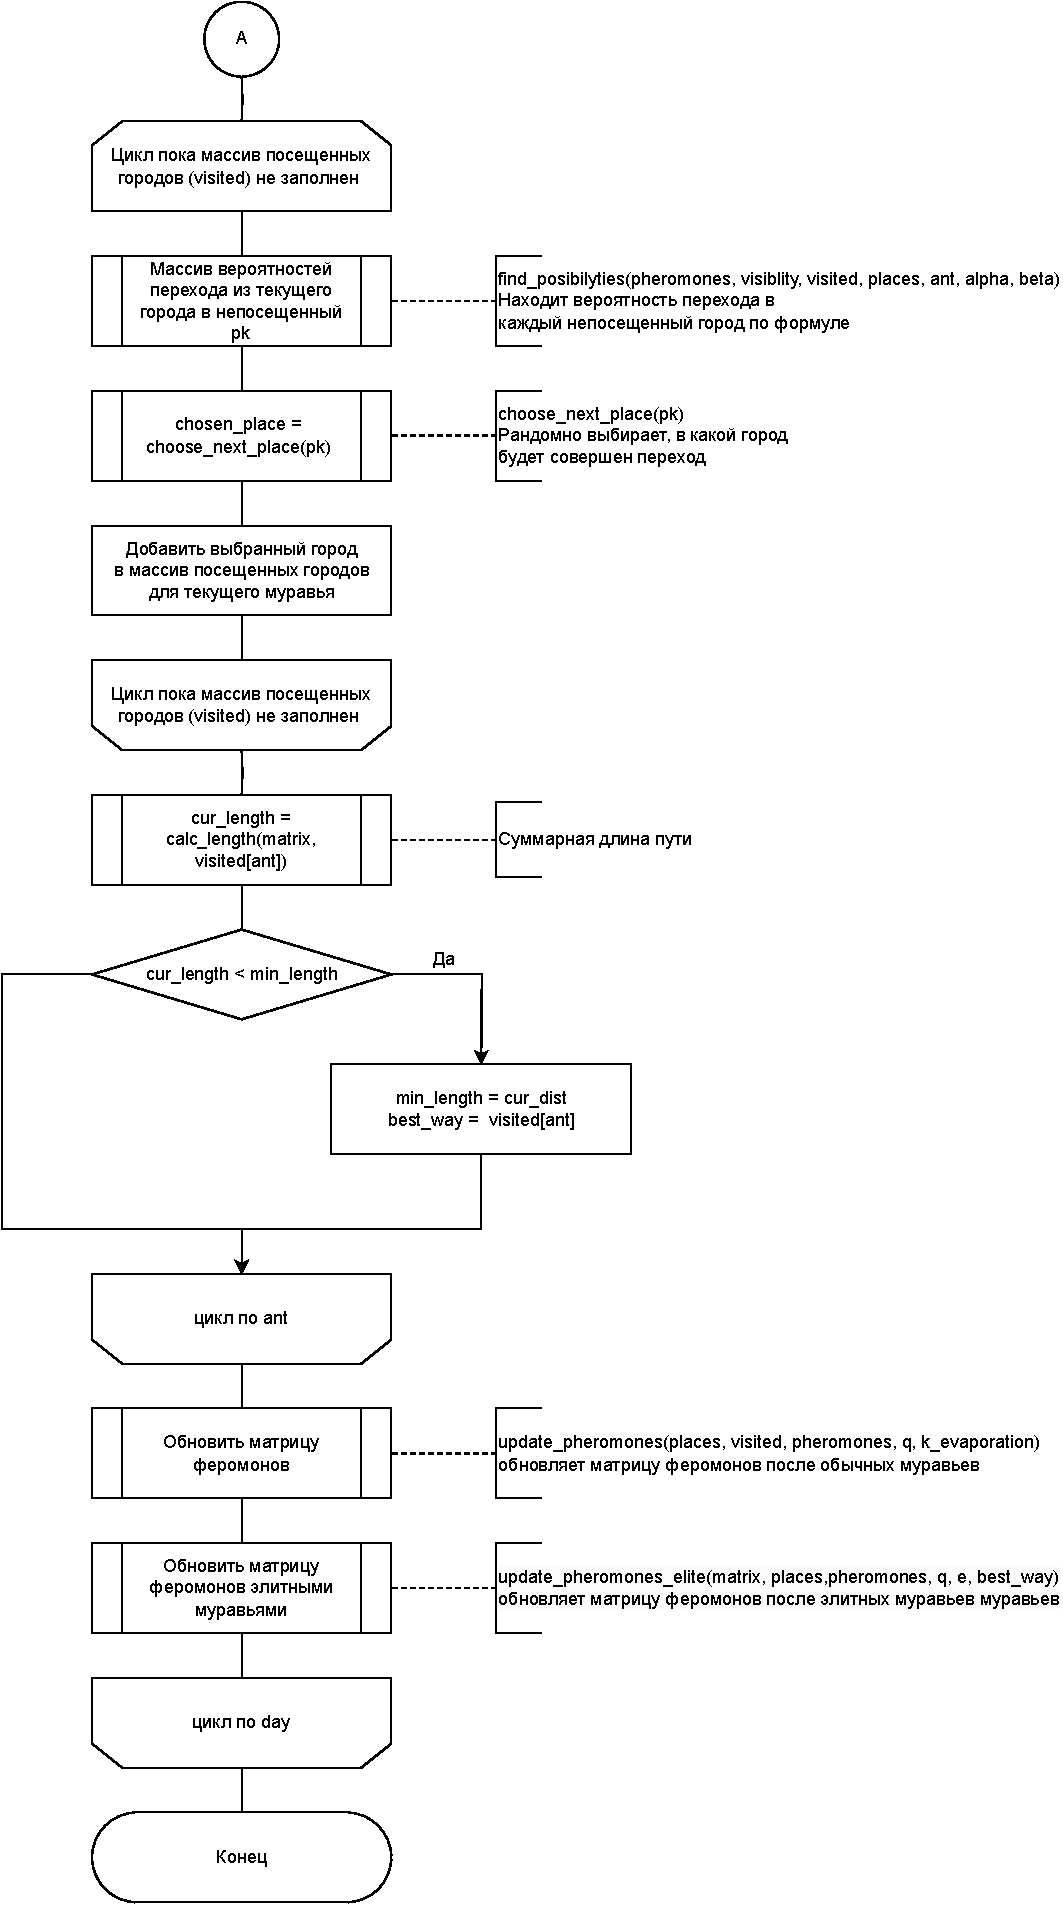
\includegraphics[width=0.8\linewidth]{img/ant2}
	\caption{Схема муравьиного алгоритма (часть 2)}
	\label{fig:ant2}
\end{figure}
\begin{figure}[h!]
	\centering
	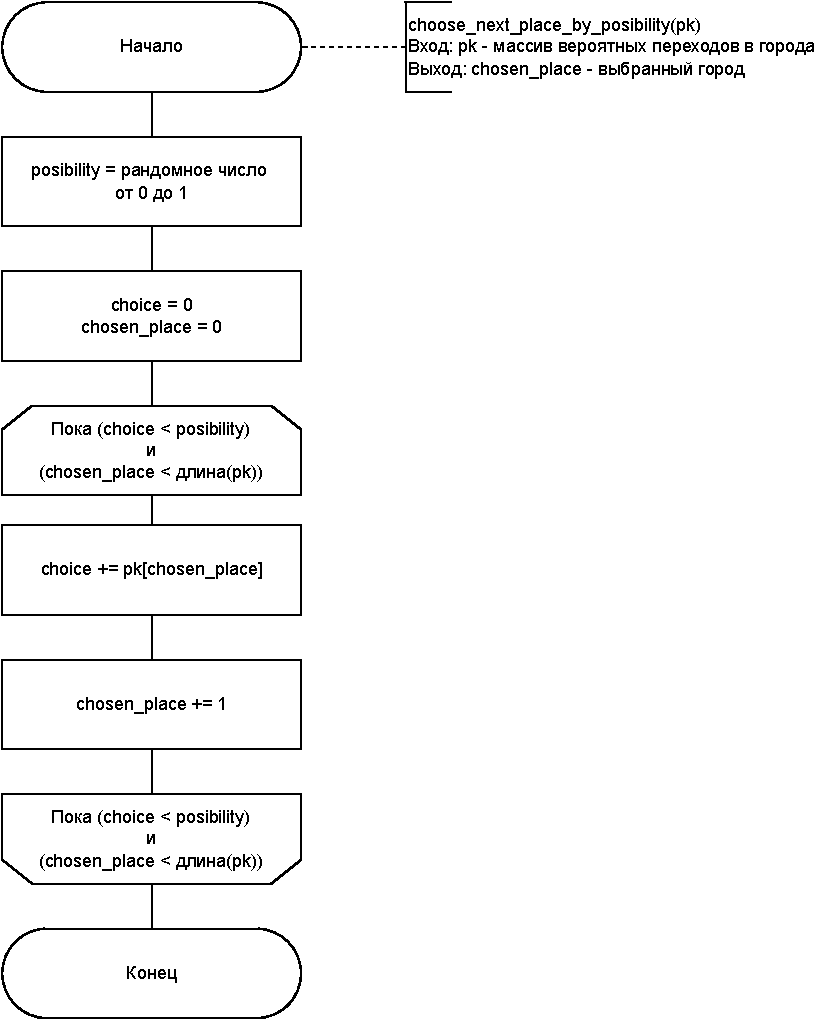
\includegraphics[width=0.9\linewidth]{img/ant_choose}
	\caption{Схема алгоритма нахождения массива вероятностных переходов в непосещенные города}
	\label{fig:ant_choose}
\end{figure}
\begin{figure}[h!]
	\centering
	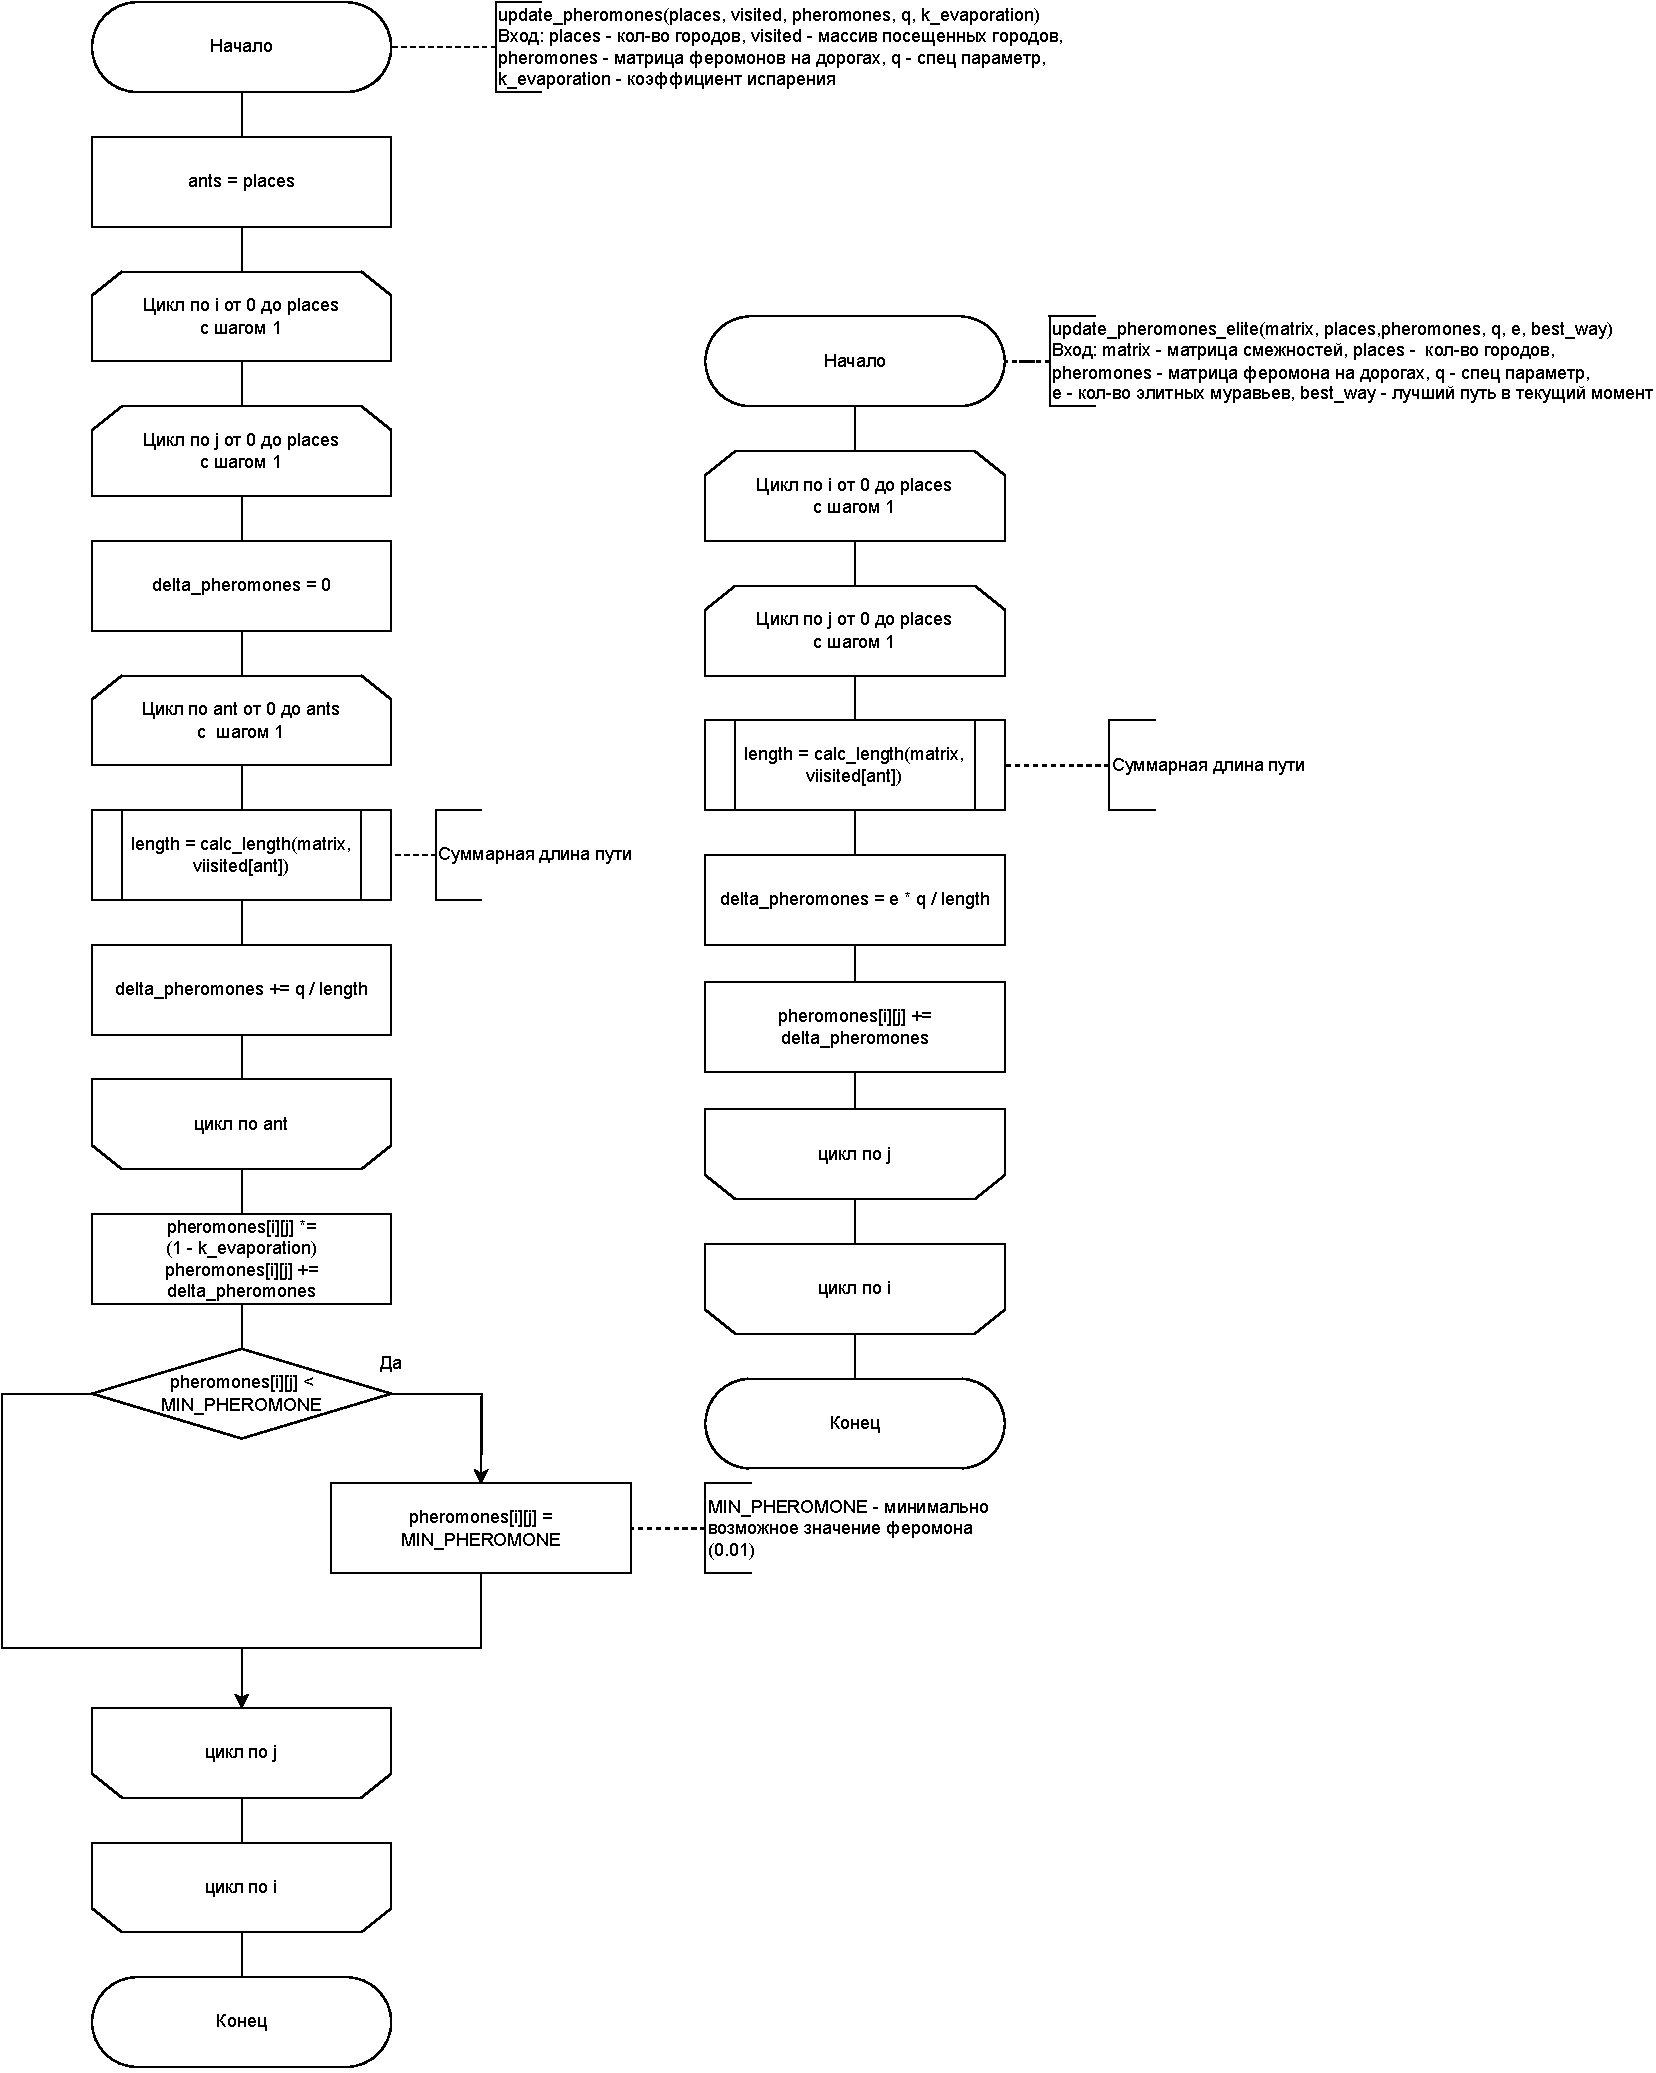
\includegraphics[width=\linewidth]{img/ant_phero}
	\caption{Схема алгоритмов обновления матрицы феромонов}
	\label{fig:ant_phero}
\end{figure}


\section*{Вывод}

В данном разделе были представлены схемы алгоритмов, рассматриваемых в лабораторной работе и требования к программному обеспечению.
